% !TeX encoding = UTF-8
\documentclass[a4paper,,twocolumn]{article}
\usepackage{graphicx}
\usepackage{listings}
\usepackage[justification=centering]{caption}
\usepackage{subfigure}  
\usepackage{multirow}
\usepackage{balance}
\lstset{language=Matlab}
\lstset{breaklines}
\lstset{extendedchars=false}

\usepackage{amsmath,amsfonts,amsthm,amssymb}
\theoremstyle{definition}
\newtheorem{thm}{Theorem}
\newtheorem{exmp}{Example}
\newtheorem{defn}{Definition}
\newtheorem{lema}{Lemma}
\newtheorem{prop}{Proposition}
\newtheorem{coro}{Corollary}


\renewcommand{\baselinestretch}{1.25}

%------------setlength----------------%
\setlength{\textwidth}{162mm}
%\setlength{\textheight}{190mm}
\setlength{\textheight}{231mm}
\setlength{\headheight}{-0.1cm}
\setlength{\topmargin}{-0.1cm}
\setlength{\oddsidemargin}{-0cm}
\setlength{\evensidemargin}{-0cm}

\setlength\columnsep{12pt}
\setlength\columnseprule{0.4pt}

\setlength{\parskip}{1mm}
\setlength{\unitlength}{1mm}
\setlength{\parindent}{2em}

\title{Project2 - Design document}

\author{Li Zhiqi\quad3180103041}

\begin{document}
\onecolumn
\maketitle
\begin{figure}[!htp]   
	\centering
	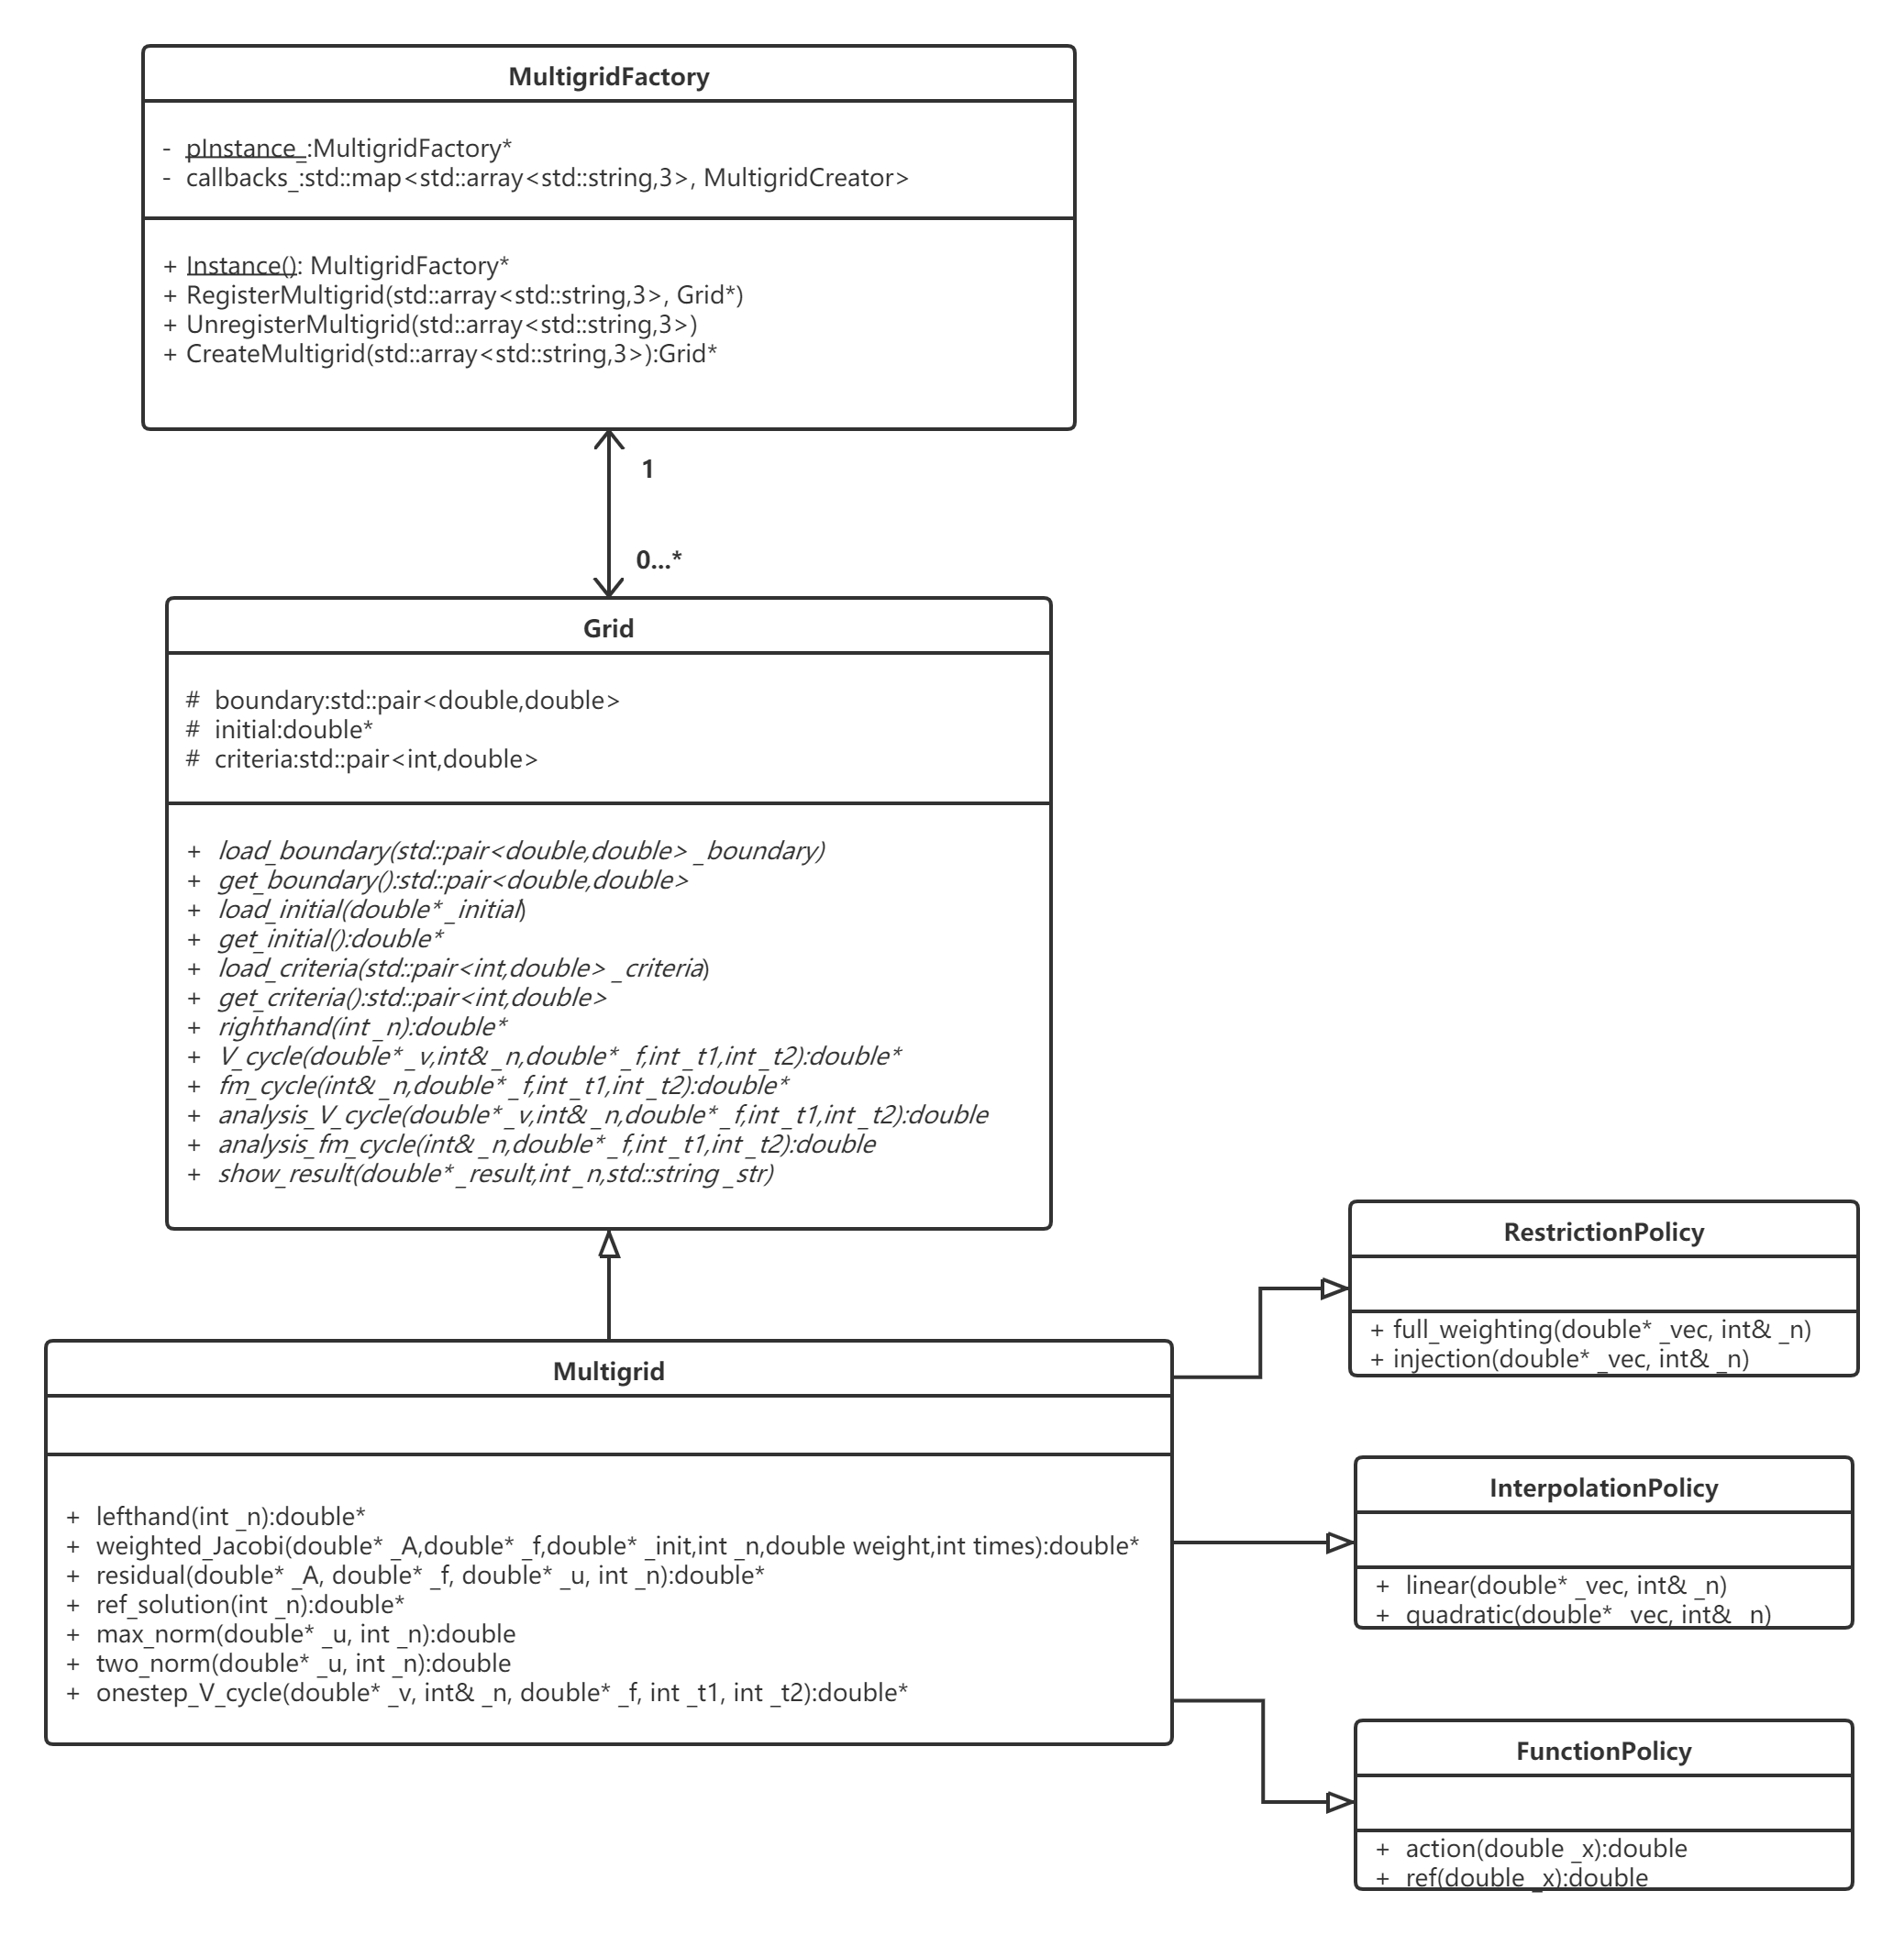
\includegraphics[width=17cm]{Pictures/Design_diagram.png}
\end{figure}
\newpage
\twocolumn
\balance
\noindent Some notes:\\\\
1.The class MultigridFactory is the factory pattern to
facilitate different choices of the policies for restriction operators,  interpolation operators and boundary conditions.\\\\
2.The class Grid is an abstract multigrid class, which has many general operations of multigrid.\\\\
3.The class Multigrid inherits from class Grid, and it's the specific multigrid we need to solve the problem. It uses weighted-Jacobi method as relaxed operator, and uses linear operation in the BLAS package to complete V-cycle and full multigrid cycle.\\\\
4.In addition, class Multigrid also inherits from class RestrictionPolicy, InterpolationPolicy and FunctionPolicy. The purpose is to enable users to choose the policies they need, while allowing programmers easily modify them by simply adding or modifying these policies.



\end{document}